\chapter{LDAPというデータベース}

本書では、メールシステムのユーザアカウント情報、マッピングなどを参照する外部データベースとして、LDAPの説明をします。
このLDAPというデータベースは、どのような思想で、どのような構造をしているのでしょうか。

\section{ディレクトリという考え方}

LDAPは、ディレクトリのサービスです。では、ディレクトリという言葉には、どのような意味があるのでしょうか。研究社の新英和中辞典では、以下のように日本語に訳してあります。

\begin{verbatim}
Directory
(特定の地区などの)住所氏名録、商工人名録
\end{verbatim}

UNIX系のOSでは、ファイルシステム上のパスをディレクトリとよんでいます。これは、いわば、ファイルの置き場所の表し方を、住所に習えたものです。

\subsection{身近なディレクトリ}

ディレクトリサービスは、場所を表すものです。身近なディレクトリサービスとして、住所があります。
例えば、コミケの会場である東京ビッグサイト会議棟の住所は、東京都江東区有明三丁目11番1です。
これをディレクトリの考え方で分解してみると、都道府県が東京都、東京都の中の区が江東区、江東区の中の町が有明、有明の中の番地が三丁目、三丁目の中の11番、11番の中の1、というようになります。

インターネットでの場所を表すURI(Unique Resoruce Location)も、同様にディレクトリです。たとえば、www.uranohoshi.exampleというホスト名は、exampleというトップレベルドメインを使っているuranohoshiというドメイン名で、ホスト名がwwwという構造です。

先ほど挙げた、ファイルシステム上のパスはどうでしょうか。たとえば、/usr/games/dmという、dm(8)のパスで考えてみましょう。これは、ルートディレクトリの先にあるusr/の、その先にあるgames/の先にあるdm、というように読みます。

\subsection{ディレクトリという考えかた}

\begin{figure}[htbp]
	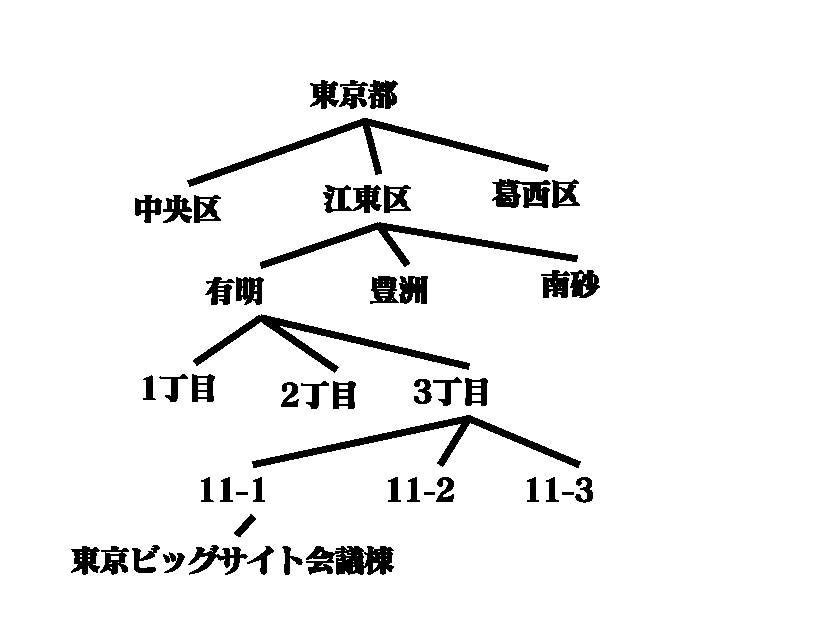
\includegraphics[width=12cm,clip]{draw/tokyo.eps}
	\caption{住所というディレクトリ}
	\label{fig:address}
\end{figure}


ここまでディレクトリの例を取り上げてきました。この、ディレクトリという考え方には特徴があります。ディレクトリは、住所のように、大きな範囲から、部分を取っていき最終的に一つの場所を表すものです。集合論的にいえば、部分空間の部分空間を選択して、最終的にその様相を特定するという考え方です。

では、なぜわざわざディレクトリという考え方をするのでしょうか。住所の例でいけば、東京都江東区有明三丁目11番1ビッグサイト会議棟と書くのではなく、東京都ビッグサイト会議棟、と書いてもいいような気がします。
では、ビッグサイト会議棟という場所をさがすとしたらどうでしょうか。

東京都の中でビッグサイト会議棟という場所を探すとしたら、東京都という範囲をすべて探す必要があります。ですが、東京都江東区の範囲で探せば、中央区や葛飾区という部分空間は探さないですみます。
更に、東京都江東区有明の範囲で探せば、江東区豊洲や江東区南砂の範囲は探さなくていいことになります。

ディレクトリは、一つのものを表すのに、全体の中のどの場所にあるかによって表現します。そして、探索の手間は、どのくらい場所を絞り込んでいるかで決まります。この絞り込みの過程を表したのが、図\ref{fig:address}です。


\subsection{木構造のグラフ表現}

\begin{figure}[htbp]
	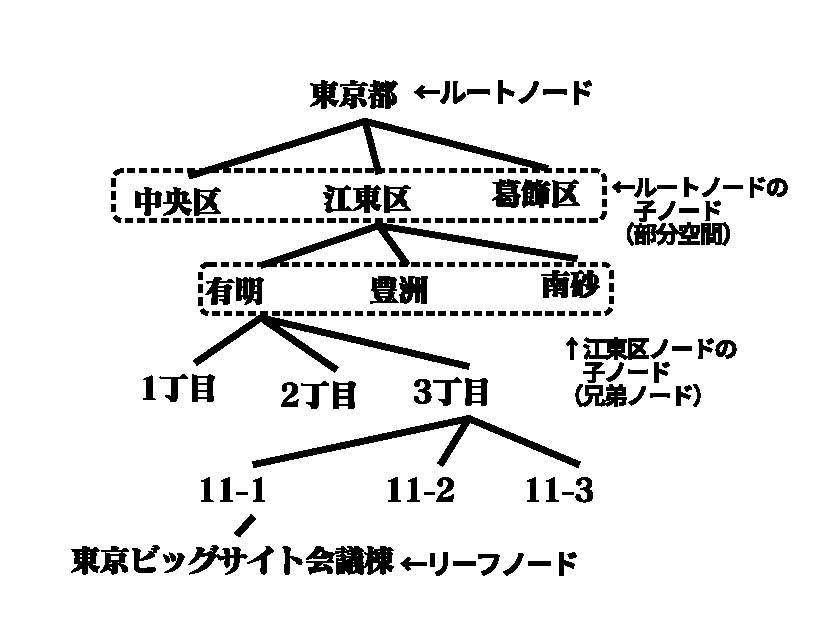
\includegraphics[width=12cm,clip]{draw/node.eps}
	\caption{ノードの種類}
	\label{fig:address}
\end{figure}

ディレクトリは、全体を表す図から、場所を絞り込んでいくイメージです。ですが、この考え方では、図として扱いにくいという欠点があります。そこで、ディレクトリは木構造のグラフを使って表現されます。

枝葉の茂った木を逆さにしたところをイメージしてください。根が一番上で、枝の端が一番下になっている状態です。その空間の全体を、その木の根におきます。もういちど、東京ビッグサイト会議棟の住所で考えてみましょう。

探索範囲の全体空間は東京都でした。なので、東京都を根に置きます。この根の部分を、ルートと呼びます。
東京都は、いくつもの市区町村からできています。これは、東京都の部分空間と考えることができます。ルートである東京都の下に、その市区町村を置きましょう。
市区町村は東京都の部分空間です。ある空間と、その部分空間は、元になった空間を上に、部分空間を下に書きます。そして、元の空間と部分空間を線で結びます。こうすると、東京都と、すべての市区町村が線で結ばれた図ができます。

この、東京都屋市区町村の一つ一つを、グラフの用語ではノード(node)と呼びます。
根元である東京都を、特にルートノード、市区町村を、ルートノードから見たとき子ノードと呼びます。また、ルートノードかどうかにかかわらず、子ノードを持っているノードを、親ノードと呼びます。
ある親ノードに対して、子ノードが一つだけ、という場合もあります。これは、親ノードの部分空間と同じ部分空間を持つ子ノードという意味になります。

市区町村は、更に町名という部分空間に分けることができます。東京都の部分空間である江東区は、有明、豊洲、南砂、というような部分空間を持っています。これらの町名は、ノード江東区から見たとき、子ノードになります。
このように、あるノードの子ノードをたどっていくことを繰り返していくと、最終的に、東京ビッグサイト会議棟というノードに行き着きます。

また、同じ親を持つノードを、兄弟ノードと呼びます。ここまでの例で言えば、有明、豊洲、南砂は同じ江東区というおやノードを持つ兄弟ノードです。

東京ビッグサイト会議棟の中のどこか、までは問うていません。そのため、東京ビッグサイト会議棟というノードは、部分空間に分割できません。つまり、子ノードを持ちません。
そのため、木の一番端である葉になぞらえて、子ノードを持たないノードをリーフノードと呼びます。

このように、全体空間から、部分空間の部分空間を選択して、何かを特定するディレクトリの考え方は、木構造のグラフであらわすことができます。

\subsection{再帰探索}



ディレクトリは、全体から部分空間を選択し、その部分空間の部分空間を選択する、それを繰り返して何かを特定します。特定の何かを探すときは、ある部分空間の部分空間の部分空間の……という繰り返しが行われます。
このように、探索の結果を対象として探索を行うことを繰り返すことを、再帰探索といいます。

東京都の中から東京ビッグサイト会議棟を探索する場合、まず、足立区の中のを探し、なければ板橋区の中を探し、と、それを繰り返していきます。
江東区の中を探す探索で、再帰探索の例をみてみましょう。部分空間有明を探索するとき、有明の部分空間である一丁目を探索します。一丁目は複数の番地に分かれていますのでその部分空間に属するリーフノードを調べ、ビッグサイト会議棟を探します。

一丁目になかったので、つぎは部分空間の二丁目を探します。二丁目の中の前部分空間のリーフノードにビッグサイトがなければ、つぎは三丁目で探します。
三丁目の部分空間11番1の子ノードに、東京ビッグサイト会議棟があります。これは、リーフノードでもあります。

このように、特定のノードが見つかるまで、すべての部分空間をリーフノードまでたどっていく探索を、再帰探索と呼んでいます。まだ、木構造の再帰探索の場合、特に、深さ優先探索、縦型探索という名前で呼ぶこともあります。


\subsection{探索の範囲と対象}

\begin{figure}[htbp]
	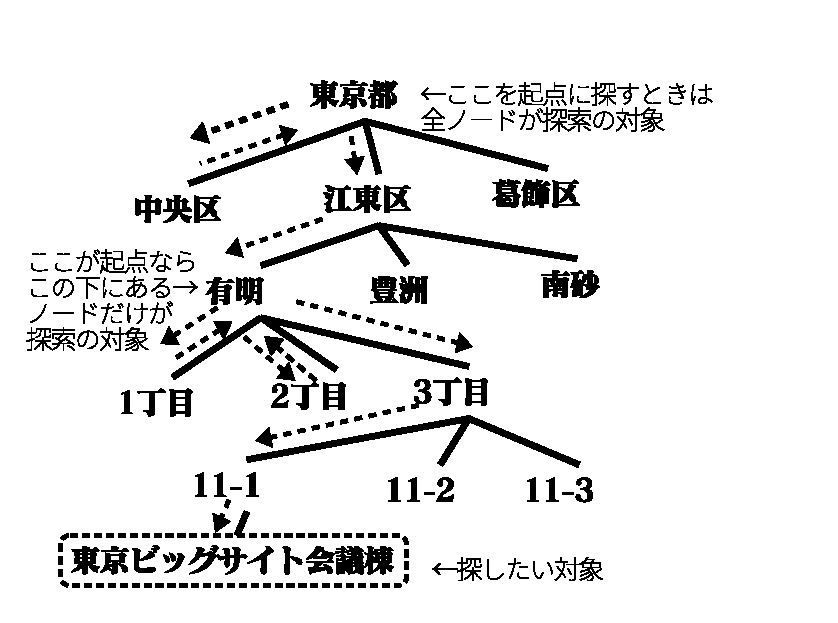
\includegraphics[width=12cm,clip]{draw/recursive.eps}
	\caption{再帰探索と探索の範囲}
	\label{fig:recursive}
\end{figure}

木構造の探索の特徴は、調べるべき部分空間があらかじめ絞れているほど、必要な計算が少なくなるということです。同じ東京ビッグサイト会議棟を探索するのでも、東京都の中から再帰探索で探すのと、東京都江東区有明の中から再帰探索で探すのでは、調べるべきリーフノードの数が大きくことなります。

また、探索の対象は、リーフノードだけではありません。木の中間にあるノードである場合もあります。たとえば、有明という町名を探索する場合、江東区の部分空間を探索した時点で、その子ノードとして有明を見つけることができます。

ただ、この場合、有明が子ノードを持つのか、リーフノードなのかという情報がありません。そのため、ルートノードの東京都から再帰探索をした場合、江東区有明を探索するまですべてのリーフノードまでを調べることになります。一方、江東区という空間の中にあることが判っている場合は、その中だけを探せばよいことになります。

\section{LDAP}

ディレクトリは全体空間から部分空間を選択して、何かを特定する考え方です。これを、データベースとして使うにはどうしたらよいでしょうか。この木構造をデータベースとして使用するのが、LDAPと言われるサービスです。
LDAPは、木構造のグラフをたどるようにして、でデータを探索します。

LDAPとは、Lightweight Directory Access Protocolの略です。もともとはDAPという複雑なディレクトリデータベースサービスを簡略化して、TCP/IPのアプリケーションとしたものです。LDAPサーバと、その情報を利用するクライアントという構成です。

\subsection{LDAPのノード}

LDAPのノードは、複数の情報を持っています。今度は、ユーザ情報がノードである場合を考えてみましょう。ユーザ情報は、ユーザ名、アカウント名、メールアドレスなど、複数の情報を持つがあります。

この一つ一つの情報を、属性(アトリビュート)と呼びます。また、その属性の具体的な値を、属性値と呼びます。
ユーザ名、メールアドレス、という情報の性質を表すのが属性、津島ヨハネ、yoshiko.tsushima@uranohoshi.exampleというような具体的な値が属性値です。
LDAPのノードは、複数の属性値をおさめる入れ物として考えることができます。


\subsection{DITとノードの場所}

LDAPのツリー構造を、DIT(Directory Information Tree)と呼びます。
では、LDAPは、DITにおける一つひとつのノードの場所どのように表すのでしょうか。そのためには、ノードを特定するのに必要な名前を定義する必要があります。

LDAPでは、この名前として、ノードに含まれる任意の属性値をひとつ選択して用います。名前として、属性と属性値をイコールで結んで表現します。
たとえば、cn=津島ヨハネ、というようにです。この名前は、兄弟ノードの中でひとつを特定するのにも用います。
ここで、cnというのは、common nameという属性です。ユーザの名前を表記するのに使う属性です。このほかに、ユーザIDにつかう、uidという属性もありますが、ここでは説明のためにcnを使います。
これは、兄弟ノード間で、同じ属性を使っても、用途が違うなら違う属性を使ってもかまいません。

\begin{figure}[htbp]
	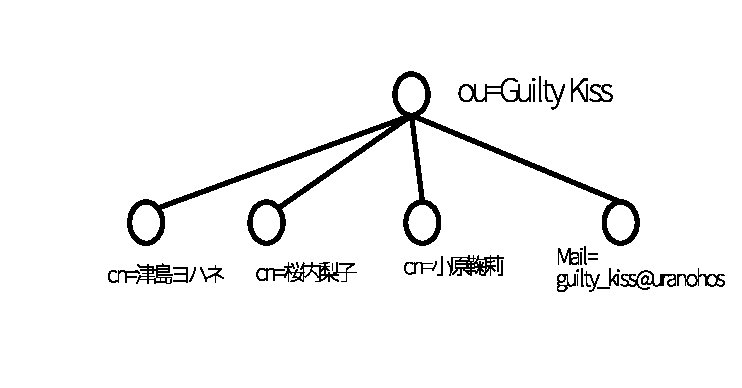
\includegraphics[width=12cm,clip]{draw/nodename.eps}
	\caption{LDAPのノードの名前}
	\label{fig:nodename}
\end{figure}

親となるノードの名前を、ou=Gullty Kissとしましょう。ouはOrganizational Unitの略で、組織の中の部署を著わすための属性です。
先ほどのcn=津島ヨハネ、の兄弟ノードとして、userName=桜内梨子、userName=小原鞠莉、というように、userNameをDNに使って区別することができます。同様に、mail=guilty\_kiss@uranohosi.exampleという名前の、メールアドレスの情報を持つノードも、兄弟ノードとしておくことができます。

\subsection{ディレクトリの中の場所をどう表すのか}

\begin{figure}[htbp]
	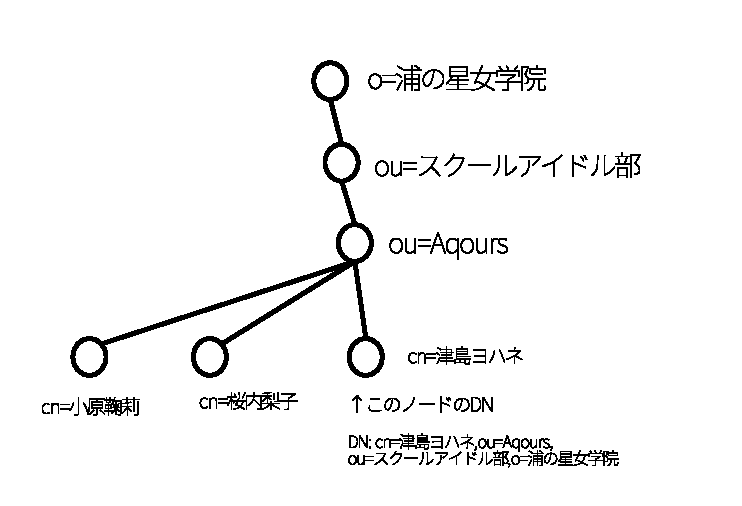
\includegraphics[width=12cm,clip]{draw/dn.eps}
	\caption{Distinguished Name}
	\label{fig:dn}
\end{figure}

LDAPでは、一つ一つのノードの名前をならべて、識別名として用います。英語のDistinguished Nameの略称であるDNがつかわれることが多いです。本書では、DNという名前を用います。

LDAPで、特定のノードがディレクトリの中のどこにあるかを表すには、目的のノードからルートノードまでのノードの名前を、カンマでつなげて記述します。たとえば、浦の星女学院のスクールアイドル部のAqoursの津島ヨハネちゃん、というDNを考えてみましょう。

浦の星女学院をルートノードとして、o=浦の星女学院、とします。このoという属性は、organizationで、組織名を著わす属性値です。
その部分空間としてスクールアイドル部を、ou=スクールアイドル部、としましょう。このouは、organizational unitで、組織内の部署を著わす属性です。
さらに、スクールアイドル部の部分空間であるAqoursを、ou~Aqoursというようにすると、津島ヨハネちゃんのDNは、このようにあらわされます。

\begin{verbatim}
DN:cn=津島ヨハネ,ou=Aqours,ou=スクールアイドル部,o=浦の星女学院
\end{verbatim}

このDNは、LDAPツリーの中では、図\ref{fig:dn}のように著わされます。
DNは、ルートノードが一番右、木の中でリーフに近いものほど左に記述されます。これは、ドメイン名などのディレクトリ名と同じ構造をしています。

\subsection{RDN}

ルートノード以外を起点として、そこからのDNを書いたものを、RDN(Relative DN)と呼びます。たとえば、先ほどの例で、ou=Aqoursを起点として記述した場合、それはRDNとなります。
また、特定のノード一つについて書いた場合も、そのノードを基準としたRDNであると言うことができます。

\subsection{同じ名前のノード}

\begin{figure}[htbp]
	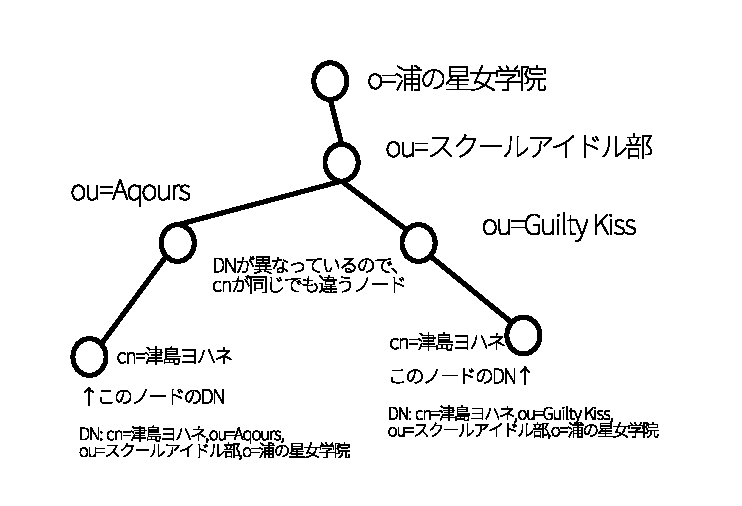
\includegraphics[width=12cm,clip]{draw/alt_dn.eps}
	\caption{DNが異なるノード}
	\label{fig:alt_dn}
\end{figure}

一つのツリーの中に、同じ名前を持つノードは存在できるのでしょうか。これは、場所を表すDNが異なれば、それは同じ名前が付いていても、違うノードとして表されます。

先ほどの例でいくのであれば、ヨハネちゃんはスクールアイドル部でGuilty Kissというユニットにも所属しています。そのため、DNでは、以下のように表すことができます。

\begin{verbatim}
DN:o=cn=津島ヨハネ,ou=Guilty Kiss,ou=スクールアイドル部,o=浦の星女学院
\end{verbatim}

この、ou=Guilty Kissの子ノードであるcn=津島ヨハネ、は、さきほどの、ou=Aqoursの子ノードであるcn=津島ヨハネとは異なるノードになります。ノードの名前は同じですが、DNとしてあらわされる場所が異なるためです。
ノードの一意性は、そのノードのDNが一位であることと同じです。DNが異なれば、それは違う存在になります。

これは、一つのノードは、親を持たないルートノードであるか、一つの親しかもてないということを表しています。これは木構造のLDAPの制限です。cn=津島ヨハネ、というノードは、ou=Aqoursとou=Guilty Kissという二つの親を持つことはできません。
もし複数の親があると、DNを特定することができなくなるためです。また、図\ref{fig:error}でわかるように、グラフが木構造にならなくなります。

\begin{figure}[htbp]
	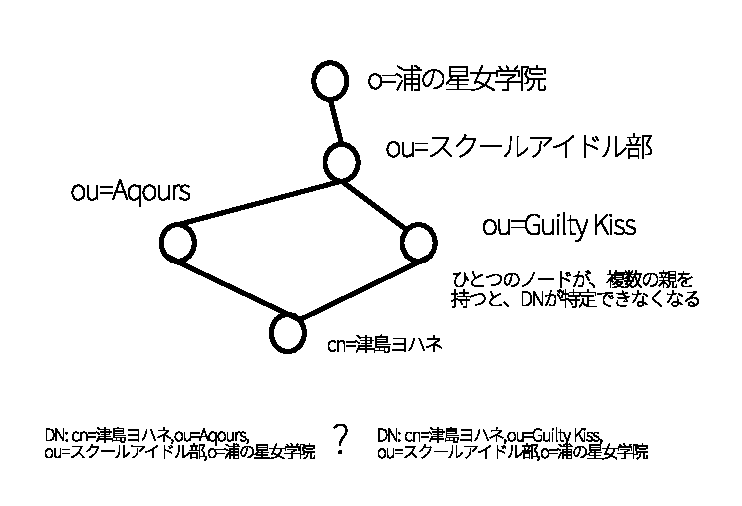
\includegraphics[width=12cm,clip]{draw/error.eps}
	\caption{ノードの親は複数あってはならない}
	\label{fig:error}
\end{figure}
